\documentclass[runningheads,a4paper]{llncs}

\usepackage[portuguese]{babel}
\usepackage{amssymb}
\setcounter{tocdepth}{3}
\usepackage{graphicx}
\usepackage[utf8]{inputenc}

\usepackage{url}
\urldef{\mailsa}\path|{alfred.hofmann, ursula.barth, ingrid.haas, frank.holzwarth,|
\newcommand{\keywords}[1]{\par\addvspace\baselineskip
\newcommand{\tab}{\hspace*{2em}}
\noindent\keywordname\enspace\ignorespaces#1}

\begin{document}


\mainmatter  % start of an individual contribution

% first the title is needed
\title{Plano de Trabalhos para Dissertação de Mestrado\\
Toolkit para análise e restauro musical
}

% a short form should be given in case it is too long for the running head
\titlerunning{Plano de Trabalhos para Dissertação de Mestrado}

% the name(s) of the author(s) follow(s) next
%
% NB: Chinese authors should write their first names(s) in front of
% their surnames. This ensures that the names appear correctly in
% the running heads and the author index.
%
\author{Bruno Miguel Correia Azevedo}
%
\authorrunning{Bruno Miguel Correia Azevedo}
% (feature abused for this document to repeat the title also on left hand pages)

% the affiliations are given next; don't give your e-mail address
% unless you accept that it will be published
\institute{Departamento de Informática,\\
Universidade do Minho\\
pg19819@alunos.uminho.pt\\
}

%
% NB: a more complex sample for affiliations and the mapping to the
% corresponding authors can be found in the file "llncs.dem"
% (search for the string "\mainmatter" where a contribution starts).
% "llncs.dem" accompanies the document class "llncs.cls".
%

\toctitle{Plano de Trabalhos para Dissertação de Mestrado}
\tocauthor{Toolkit para análise e restauro musical}
\maketitle


Estudante: Bruno Miguel Correia Azevedo\\

Orientador: José João Dias de Almeida\\

Local de trabalho: Departamento de Informática, Universidade do Minho\\


\begin{abstract}
Presentemente, plataformas cooperativas para edição de partituras musicais, como a Wiki::Score que
utiliza a notação abc, não têm à sua disposição utilitários de avaliação e deteção de erros, nem
ferramentas que auxiliem a musicologia. Esta carência impede os utilizadores de tirarem o melhor
partido dessas plataformas e proporciona um sentimento de limitação na composição e transcrição de
partituras.

Para colmatar estas falhas, e adotando a filosofia utilizada pelo sistema operativo Unix, criar-se-á
um toolkit, em que cada ferramenta trata um problema individualmente, como a deteção e correção de
erros sintáticos, léxicos, entre outros. Para que estas ferramentas tenham uma componente
musicológica como a análise tonal e deteção de padrões, é necessária a construção de corpora de
obras musicais, onde, após análise, é possível extrair conhecimento que será integrado nas
ferramentas criadas ou exibido ao utilizador num formato específico.
\keywords{notação abc, toolkit, musicologia, validação e deteção de erros, corpora}
\end{abstract}


\section{Enquadramento}

\subsection{Notação Textual Musical}
Toda a música precisa de ser escrita antes de ser lida, percebida e executada por qualquer músico e,
para que tal seja possível, um sistema de notação foi desenvolvido que proporciona aos músicos a
informação necessária para reproduzir a música tal como o compositor pretendia. A notação musical
consiste em qualquer sistema que representa música auditivamente perceptível através da utilização
de símbolos escritos. Essa utilização de formatos simbólicos e abstratos melhora a capacidade e o
raciocínio da música, pois dá uma liberdade de expressão maior ao compositor e proporciona uma mais
fácil leitura ao executante. \\
Com a integração de computadores e música, uma variedade de formatos de ficheiro e notações
textuais\footnote{exemplo: lilypond, musicXML, abc} começaram a surgir para armazenar notação. Um
exemplo de formato é a \textbf{notação ABC}. Trata-se de um sistema concebido para definir e anotar
música em formato de texto simples, inicialmente para \textit{folk} e melodias tradicionais com
origem na Europa Ocidental, que pode ser escrita numa única pauta em notação clássica standard.
Desde a sua introdução nos finais de 1991, tem-se vindo a tornar bastante popular, existindo dezenas
de milhares de músicas em abc e muitas ferramentas de software que conseguem ler a notação e ainda
processá-la para notação gráfica ou reproduzi-la. Uma das características prinicipais e
diferenciadores desta notação é o facto de esta também poder ser lida pelo Homem, ou seja, é
possível reproduzir uma música diretamente da notação sem ter que a processar e exibir.

\subsection{Processamento de Notação Textual Musical}
Cada vez mais, a musicologia auxiliada por computador é uma realidade, o que leva a que exista uma
maior investigação em algumas áreas da música como a análise tonal e a composição. Da mesma forma, o
que se pretende é uma contribuição para esta área da investigação, proporcionando ferramentas que
auxiliem a análise, a deteção de erros, o restauro de documentos, etc, para documentos abc. De
momento, a composição não se encontra abrangida no âmbito desta dissertação, no entanto, é uma
componente bastante interessante para se abordar.

\subsection{Filosofia Unix}
Nos anos 70, o sistema operativo Unix surgia e com ele uma nova filosofia que assentava na ideia de
que ferramentas robustas e complexas não tinham grande interesse, ao invés de ferramentas de menor
escala, simples e eficazes que tratam, tipicamente, um único problema e cuja combinação entre si
fosse possível. O método principal de interação com o sistema é a linha de comandos onde um
utilizador corre comandos e programas o que torna o método de traballho bastante poderoso e
flexível, porque dessa forma é possível compô-los e executá-los automaticamente. Ainda hoje, este
método de trabalho é utilizado pela maioria dos utilizadores avançados e administradores Unix.\\

Muitos dos comandos Unix, executam funcionalidades de dimensão reduzida e têm como input e output um
tipo de dados comum, o que permite a articulação de comandos. Tal filosofia é facilmente aplicável a
partituras digitais, nomeadamente, a ficheiros de notação musical. Existem alguns comandos Unix cuja
funcionalidade pode facilmente ser adaptada à realidade das partituras, tais como:
\begin{itemize}
  \item \textbf{grep:} imprime as linhas de um ficheiro que correspondam a um padrão;\\
poder-se-ia, por exemplo, imprimir sequências melódicas que correspondessem a um padrão, padrão esse
que poderia ser um sequência de intervalos melódicos, ou uma sequência rítmica
\item \textbf{diff:} compara ficheiros linha a linha;\\
poder-se-ia comparar dois ficheiros voz a voz
\end{itemize}

\subsection{Áreas de aplicação}
Algumas das atividades que maior benefício retiram deste toolkit são:
\begin{description}
\item[Wikis musicais]
Wikis que lidam com a edição de partituras musicais. Exemplo: Wiki::Score
\item[Voluntariado cultural e cooperativo]
Ambientes como as wikis, onde a edição de documentos ocorre em cooperação com vários elementos
concorrentemente. Exemplo: Wiki::Score
\item[Transcrições de obras]
Por vezes, ocorrem erros variados no decorrer da transcrição de uma obra e nem sempre esses erros
são facilmente detetáveis.
\item[Legados musicais]
\item[Análise e composição musical simples]
Por exemplo, através da deteção de certos padrões em determinado estilo musical, é possível avaliar
se determinada composição obedece a algumas facetas características desse estilo.

\end{description}

%\subsection{Dificuldades}


\section{Objetivos}
Dado o contexto descrito no capítulo anterior, pretendemos criar um toolkit, ou seja, um conjunto de
ferramentas que, individualmente, resolvem um problema específico e cujos resultados possam ser
articulados. Este toolkit tem como objetivo principal o aumento da abstração e da granularidade da
informação musical aplicado a problemas de musicologia, de modo a que de informação musical se possa
gerar conhecimento, por exemplo, em forma de vistas eficazes sobre a informação simbólica.

\subsection*{Toolkit}
As ferramentas irão cobrir os vários problemas de Processamento de Notação Textual Musical:
\begin{enumerate}
\item Validação automática de documentos de notação musical, assim como, deteção de erros
existentes. Esses erros podem ser relativos a: 
\begin{itemize}
\item \textbf{sintaxe}\\
exemplo: tempos por compasso, armações de clave diferentes entre vozes
\item \textbf{léxico}\\
exemplo: utilização indevida de símbolos
\item \textbf{desalinhamento}\\
exemplo: Disparidade de vozes devido a erros de transcrição
\item \textbf{utilização suspeita de elementos musicais em geral}\\
exemplo: dado o estilo musical ou outras características identificadas na peça, a utilização de
acordes fora do contexto ou acordes demasiado grandes (instrumento: canto)
\end{itemize}
\item Correção dos erros detetados. Exemplo:
\begin{itemize}
\item Para os erros de sintaxe, no caso da existência de várias pausas consecutivas, poder-se-á
sugerir a junção das mesmas por compasso. Se uma mudança da armação de clave ocorre apenas numa voz
quando o esperado é uma mudança em todas as vozes, então essa mudança é refletida nas restantes
vozes.
\item Para erros léxicos, é bastante comum existirem erros ortográficos ou de capitalização em
palavras reservadas, nesse caso, a correção automática é esperada.
\end{itemize}

\item Filtros diversos baseados na metáfora Unix como: grep, diff, cut, paste, cat, join, sed, entre
outros, musicais.
\end{enumerate}

\subsection*{Corpora Musical}
Outro objetivo passa pela possibilidade de calcular a diferença entre o que é considerado padrão, de
aferir o que é esperado (regra, habitual), de calcular semelhanças entre obras, de fazer comparações
estatísticas e para que tal seja exequível é necessário que existam casos de exemplo.

Esses casos de exemplo não são mais do que um corpus musical que contém um conjunto de metadados
rico e por isso a construção do mesmo torna-se um objetivo essencial. Com a existência deste corpus
será possível às ferramentas criadas tirarem partido de informação calculada na análise de corpora
e, desta forma, existir uma maior integração entre as ferramentas do toolkit.\\

Com base nos corpora existentes e, tal como foi referido no ponto anterior, pretende-se calcular
dados estatísticos resultantes da análise dos mesmos, para isso, ferramentas de cálculo estatístico
serão construídas.\\

\subsection*{Representação de informação musical}
Um estudo sobre representações internas de informação musical irá ser feito para que se possa
relacionar e comparar diferentes representações e chegar a uma conclusão quanto à implementação que
será utilizada no nosso toolkit.\\

Devido ao grande avanço na área da musicologia auxiliada por computador, existem várias ferramentas
que tentam dar o seu contributo na área e para que possa haver uma melhor percepção dos avanços que
foram feitos até então, um estudo dessas ferramentas será feito.\\

\subsection*{Visualização de informação musical}
Após feita a análise de qualquer obra através do toolkit é necessário mostrar o resultado. Um
resultado gráfico é ideal para que a sua percepção seja mais fácil e assim possa revelar alguma
faceta da música, por exemplo, o desenvolvimento tonal que a música tem do início ao fim. Desta
forma, estudar-se-á que facetas da música interessam ao utilizador para o auxiliar na análise e o
melhor formato para as exibir.

\section{Metodologia de trabalho}
Para o desenvolvimento do sistema e para a escrita da dissertação serão utilizados os seguintes
métodos:
\begin{itemize}
\item Pesquisa bibliográfica;
\item Metodologias ágeis de desenvolvimento;
\item Desenvolvimento suportado por testes;
\item Extração e aprendizagem de informação baseada em corpora
\end{itemize}

\section{Calendarização}
O trabalho desenrolar-se-á no ano lectivo de 2012/2013, com uma duração estimada de 9 meses. A
escrita da dissertação irá decorrer em paralelo com as actividades descritas nesta proposta de
trabalho, de acordo com o seguinte calendário:
\begin{enumerate}
\item \textbf{Pesquisa bibliográfica}. Pesquisa e estudo de publicações relacionadas com o tema da
dissertação: abc, representações internas, ferramentas, etc...
\item \textbf{Criação de corpora} com metadados ricos.
\item \textbf{Desenvolvimento de ferramentas para estatística musical}
\item \textbf{Desenvolvimento de ferramentas para análise}
\item \textbf{Estudo da viabilidade da componente de composição}. Componente abordada nos capítulos
anteriores e que se revela, à partida, complexa.
\item \textbf{Redação da dissertação}
\end{enumerate}

\begin{figure}[htb]
     \center { 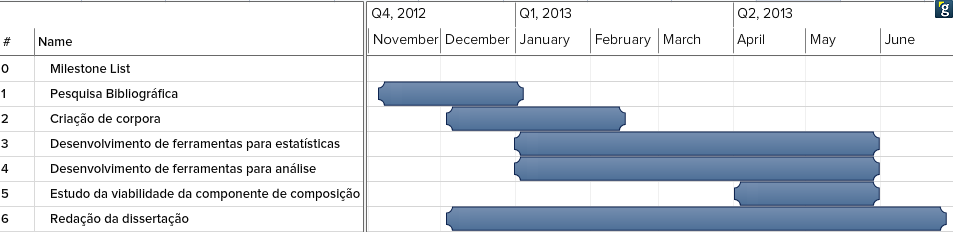
\includegraphics[width=\textwidth]{gantt.png}}
     \caption{Calendarização através de um diagrama de Gantt}
\end{figure}
\newpage
\bibliographystyle{plain}
\nocite*{}
\bibliography{proposta}
\end{document}
